% - intro: motivation fusionize, presentation of implementation of paper
%   concept with a real faas platfrom, nuclio
%   - use figs 2 and 3 from paper

\section{Fusionize}\label{sec:fusionize}

%this section goes into more detail of the briefly introduced Fusionize paper
%it presents the implementation strategy of this paper and explains all
%components
%ti presents a guide of how a user setups their Fusionizer-enabled tasks

This section further examines the \textsc{Fusionize} paper that was briefly
introduced earlier. It details the implementation strategy for the paper's
concepts and clarifies its various components. Additionally, a user guide is
provided to assist the process of setting up their Fusionizer-enabled tasks.

\subsection{Concept}

\textsc{Fusionize}, by Schirmer et al. \cite{schirmer2023fusionize} is a
feedback-driven framework that automates the setup of composite task-based
applications on cloud FaaS platforms. As outlined in Figure
\ref{fig:fusionize_highlvl}, it takes unchanged FaaS tasks and enhances their
performance and cost-efficiency by iteratively modifying their deployment
configuration and inlining tasks based on monitored performance.

\begin{figure}
    \centering
    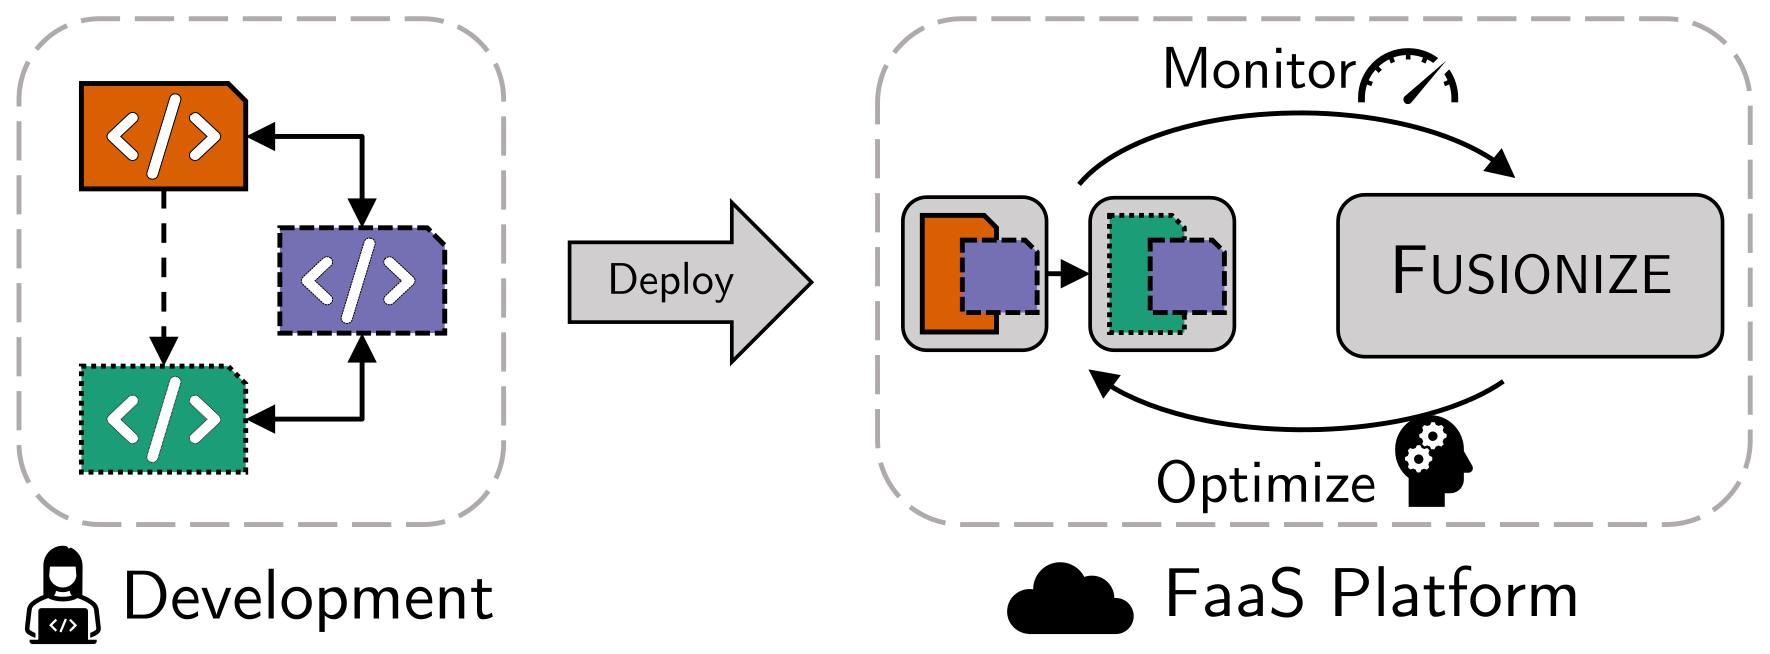
\includegraphics[width=\linewidth]{../figures/fusionize_highlvl}
    \caption{
        High-level overview of \textsc{Fusionize} \cite{schirmer2023fusionize}.
        \textsc{Fusionize} optimizes FaaS tasks' performance and cost by
        altering deployment configurations and inlining tasks within FaaS
        functions.
    }
    \label{fig:fusionize_highlvl}
\end{figure}

The concept of inlining from compiler theory is used to expand remote FaaS
function calls with task source code where beneficial, a concept known as
function fusion. Function fusion can reduce remote call overheads and confine
cold start cascades.

Using the familiar FaaS programming model, \textsc{Fusionize} processes current
FaaS applications and infers their call patterns, cost efficiency, and
performance from live execution behavior. It then continuously optimizes the
application setup for cost efficiency and end-to-end performance. If application
behavior changes, \textsc{Fusionize} can automatically adapt to this new
environment and optimize further.

In the context of \textsc{Fusionize}, \emph{task} refers to any software
function that developers construct, while \emph{function} denotes an executable
deployment artifact. Each function contains a single \emph{fusion group}, which
is a set of tasks executed as part of the function.

\subsection{Implementation Overview}

The initial concept for implementation with Nuclio was to develop a new function
processor that would manage the inlining of functions. These would be selectable
during the function deployment phase. However, the underlying platform component
of Nuclio and its Kubernetes (k8s) implementation does not account for the
possibility of mapping multiple tasks to a single function. A consultation with
the Nuclio developers revealed that a complete rewriting of the platform would
be required to enable this functionality. This proved unrealistic within the
scope of this project for a single developer.

Instead, an independent \emph{Fusionizer} server, developed in Python, is
introduced between the user and a non-modified, \emph{vanilla} Nuclio platform.
As depicted in Figure \ref{fig:fusionizer_highlvl}, the user only interacts with
the Fusionizer server, not Nuclio directly. The server provides a REST API for
task management, adopting the same function configuration for tasks as with
deployment via Nuclio.

\begin{figure}
    \centering
    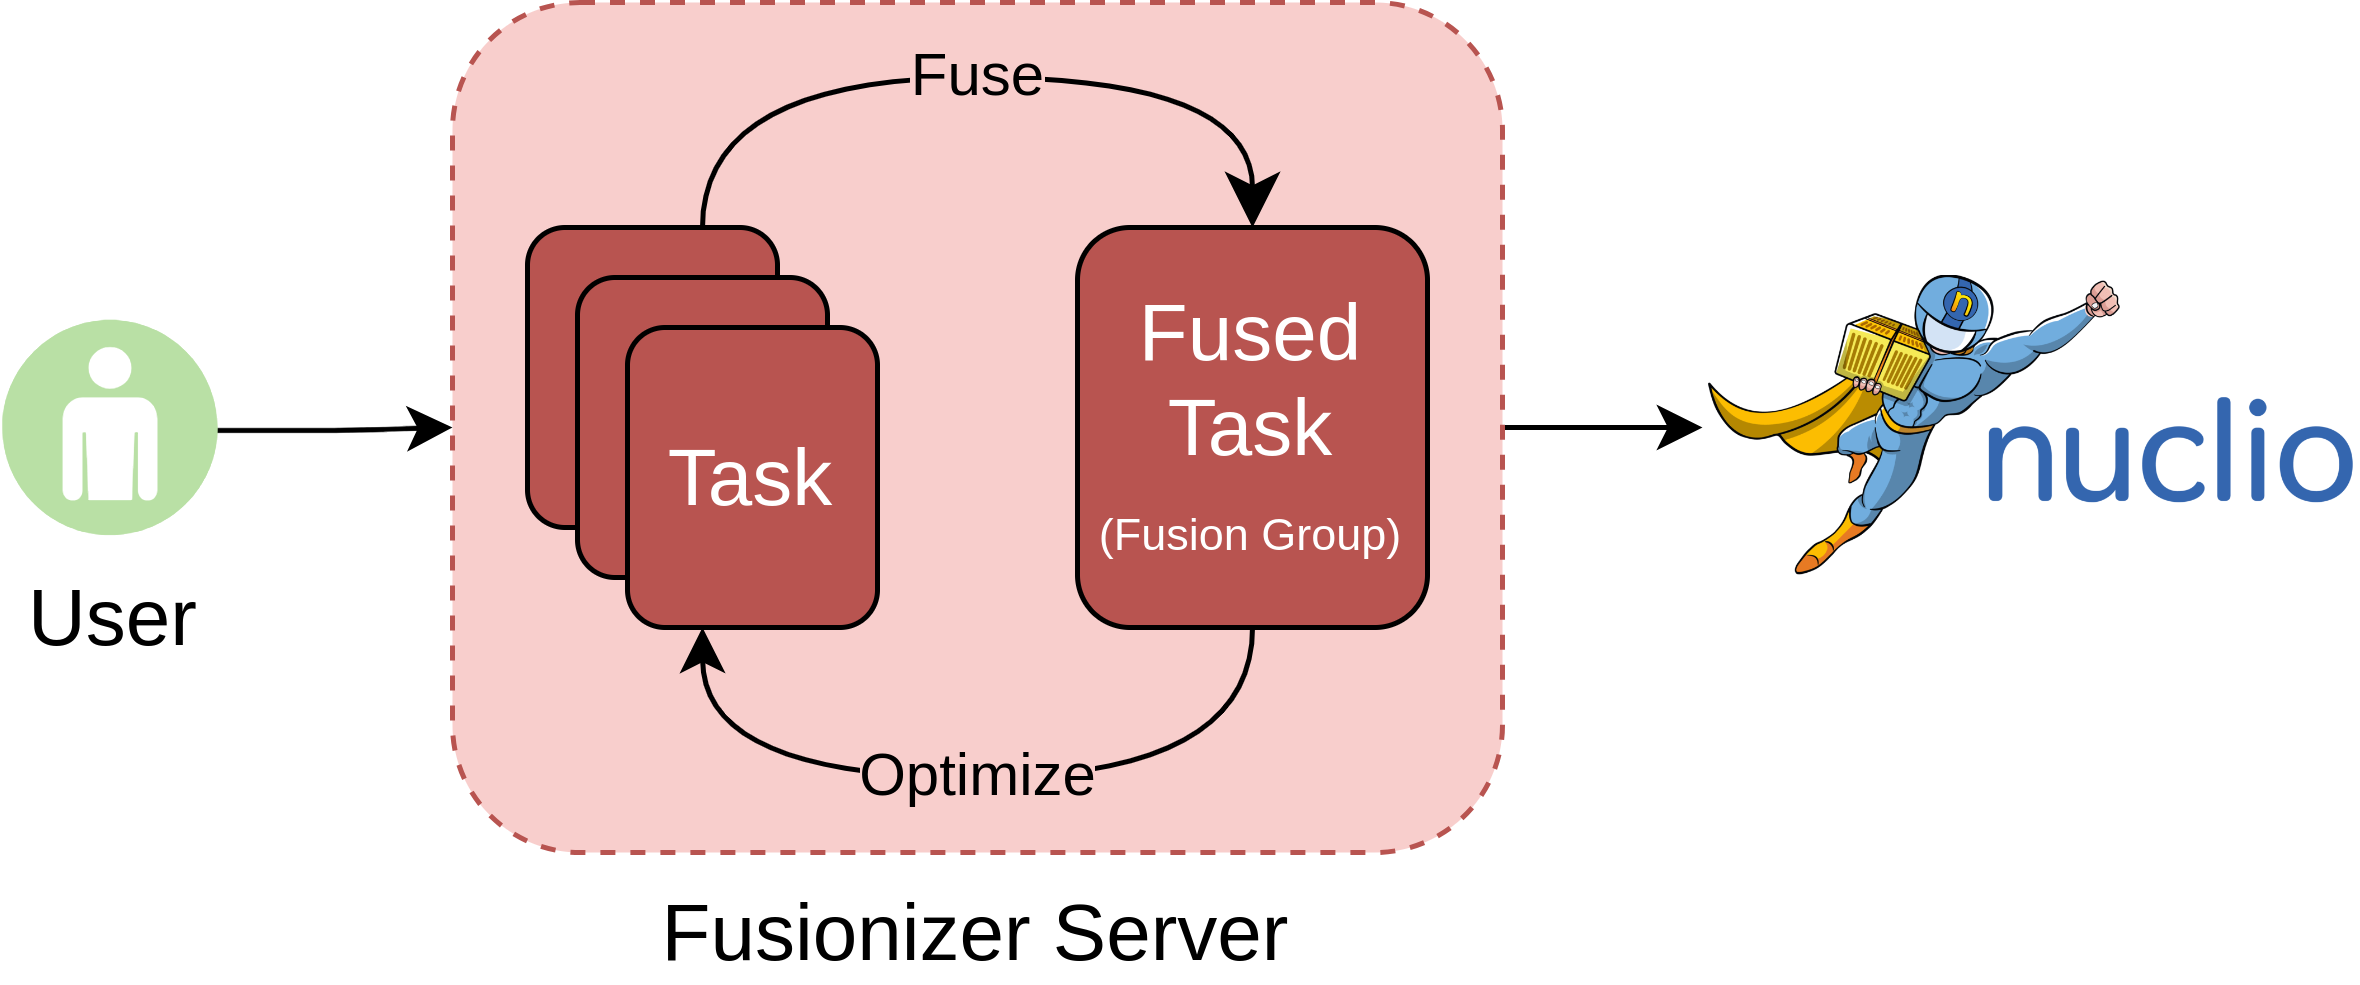
\includegraphics[width=\linewidth]{../figures/fusionizer_highlvl}
    \caption{
        High-level implementation overview. The user does not deploy or invoke
        their tasks through nuclio, but the Fusionizer server which applies the
        concepts of \textsc{Fusionize}.
    }
    \label{fig:fusionizer_highlvl}
\end{figure}

Users deploy their fine-grained application code to the Fusionizer server. The
server then groups tasks into fusion groups, according to an optimization
strategy. Each of these groups are fused into a single Nuclio function and
deployed to the platform. Each Nuclio function deployed from the Fusionizer
server contains a dispatcher component. This component routes invocation
requests from the Fusionizer server to the appropriate task. Additionally, HTTP
invocation requests between two tasks contained within the same Nuclio function,
or fusion group, are intercepted and invoked locally. To minimize network
overhead, the Fusionizer server is housed on the same machine as Nuclio. This
implementation, however, only enables the concepts presented in the paper and
does not represent any optimization strategies.

This strategy offers significant advantages as it can be executed without the
time-consuming task of comprehending and altering the existing codebase of
Nuclio. The applicability of this strategy is also not confined to Nuclio as the
single FaaS platform, as further detailed in Section X.

\subsection{Components}

This section reviews the individual components that compose the Fusionizer
server and provides a more detailed view. The overall relationship between these
components is visually represented in Figure \ref{fig:fusionizer_components}.
The main components involved in this system are the API server, the nuctl
interface, the Optimizers, the Task Fuser, and the Dispatcher.

\begin{figure}
    \centering
    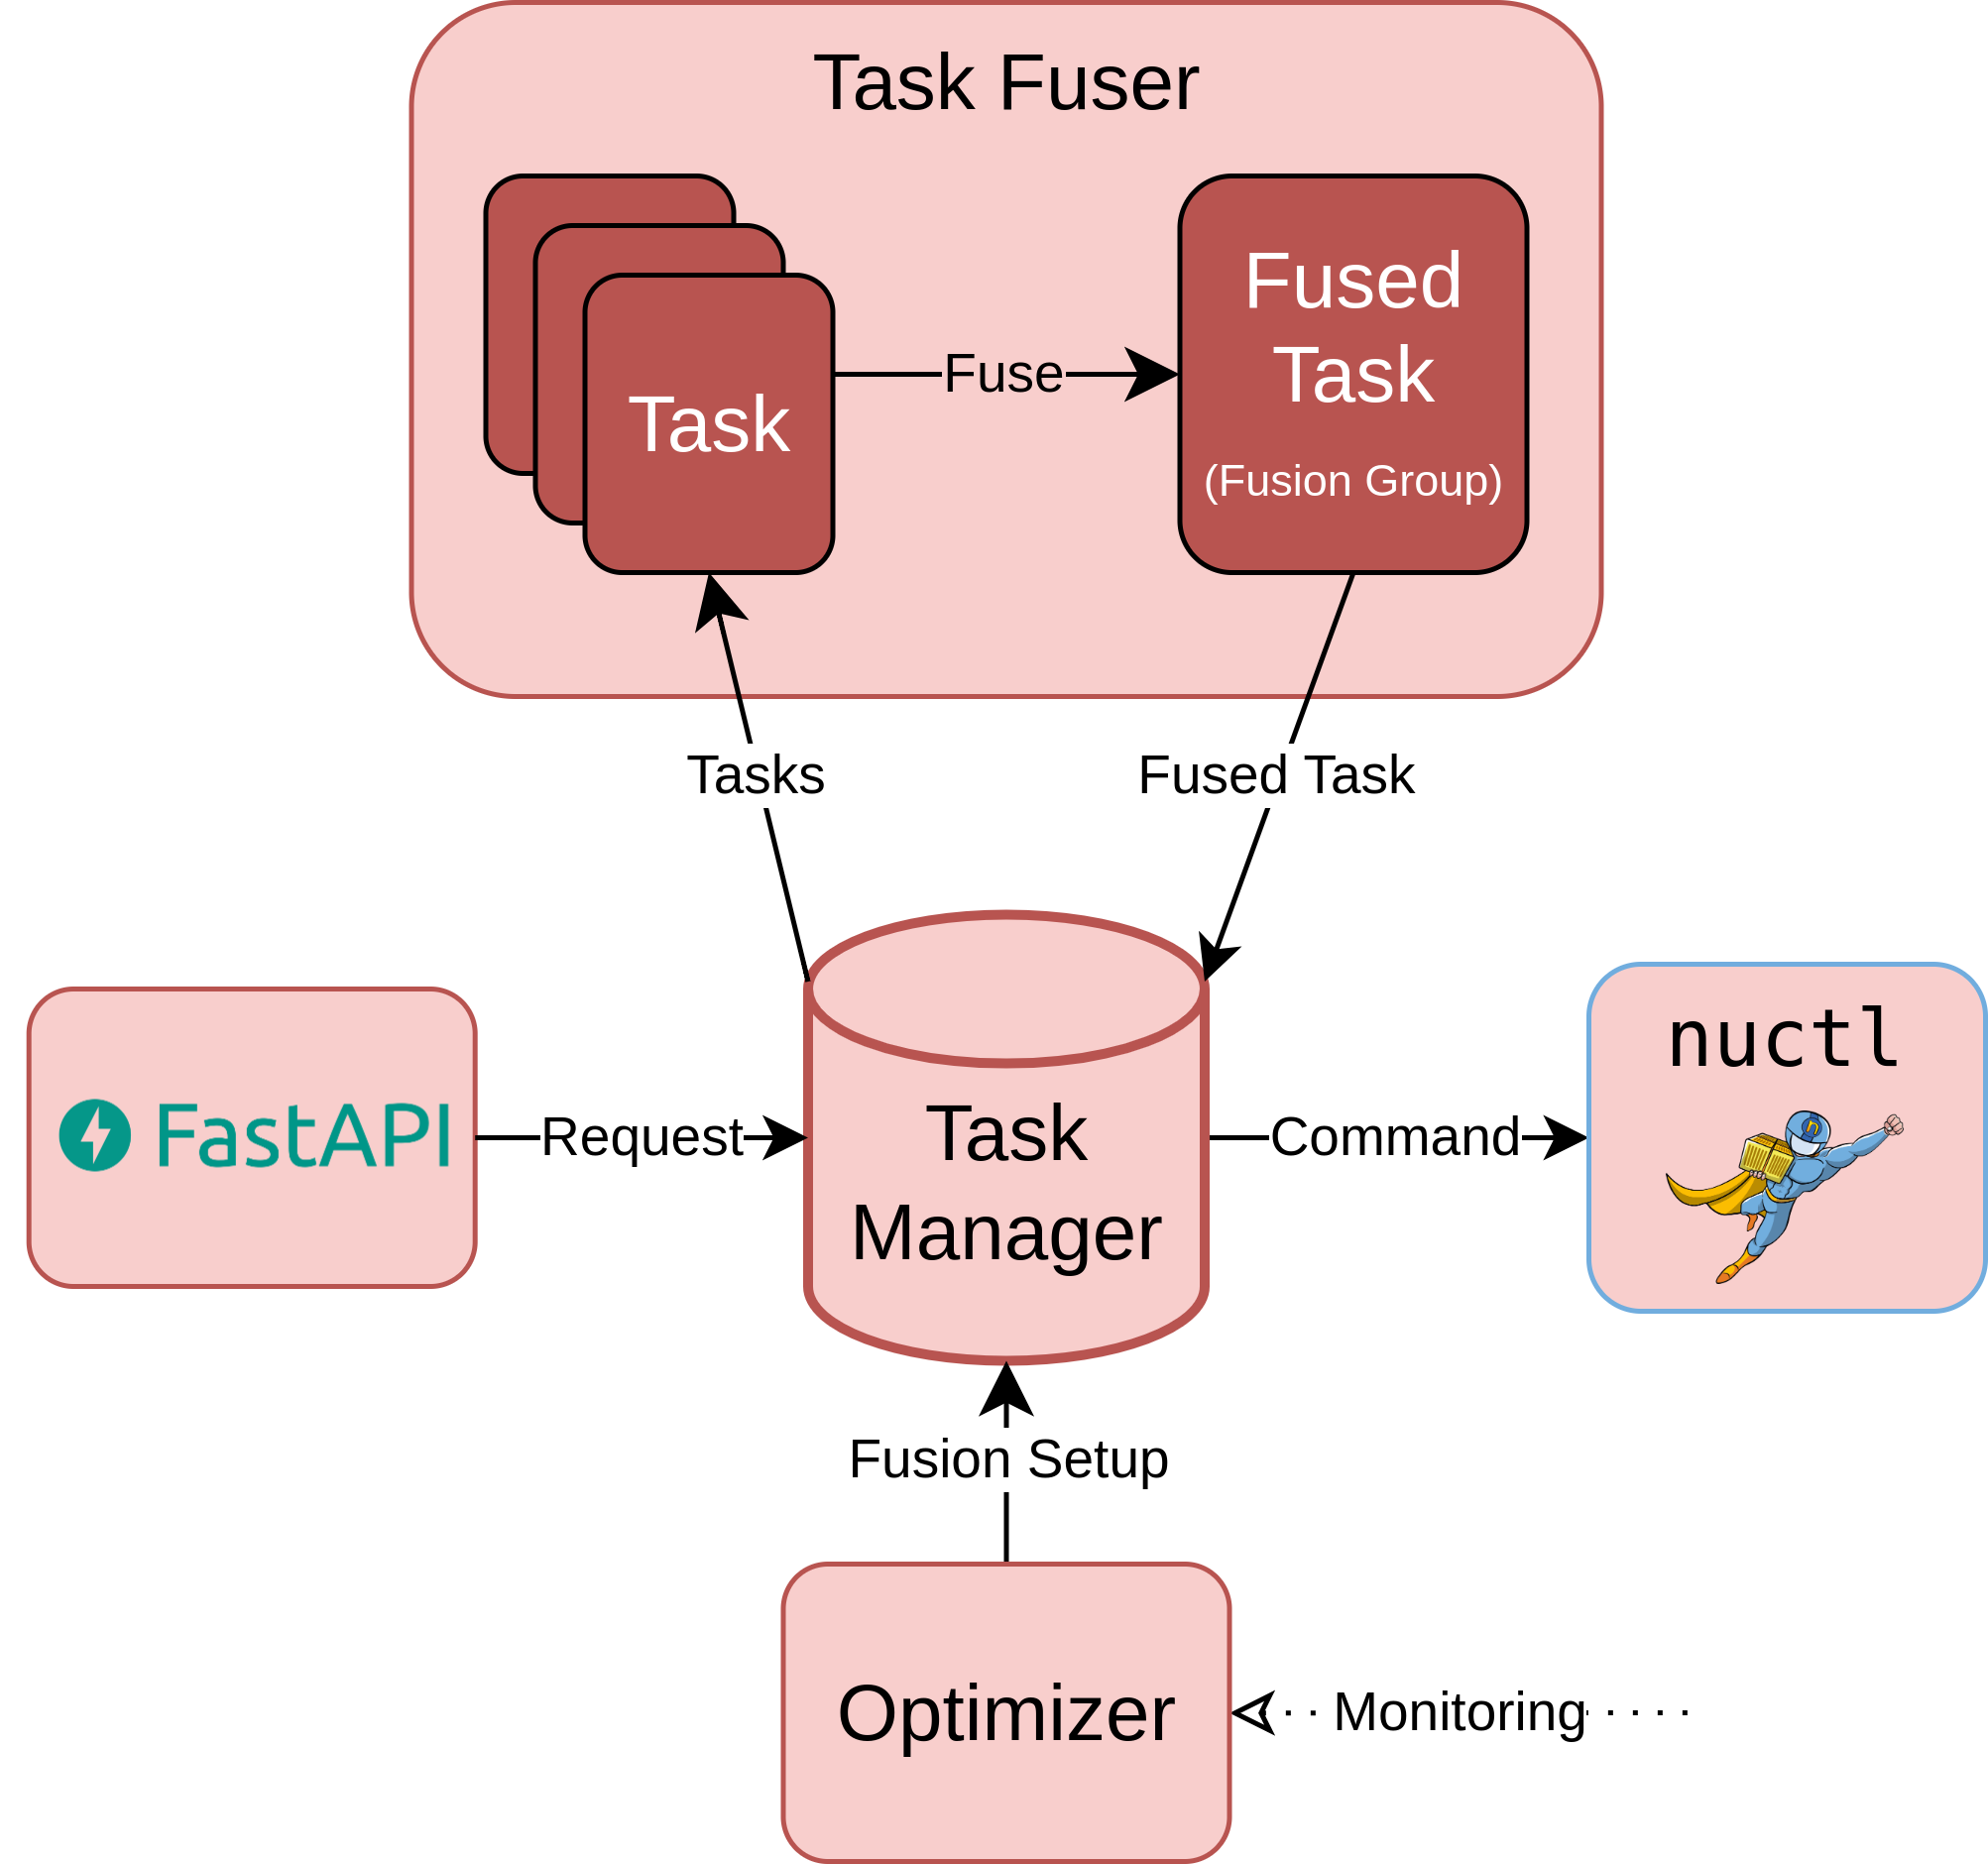
\includegraphics[width=.8\linewidth]{../figures/fusionizer_components}
    \caption{
        Fusionizer server components. The API server forwards incoming requests
        to the Task Manager. Then, following the fusion setup configured by the
        Optimizer, tasks are dispatched to the Task Fuser. Here, tasks are
        merged into a Nuclio function which is subsequently deployed through the
        nuctl interface.
    }
    \label{fig:fusionizer_components}
\end{figure}

\subsubsection{API Server}

%api server offers RESTful api to the user this FastAPI based server provides
%HTTP interface for user interaction with the fusionizer system. api can be seen
%in Table 1 the http endpoint always stays the same and is structured like
%http://<url>/<task-name>/

The API server provides a RESTful API to the user, acting as a FastAPI-based
server. It offers an HTTP interface which facilitates seamless user interaction
with the Fusionizer system. Information regarding the API can be found detailed
in Table \ref{tab:fusionizer_api}. The structure of the HTTP endpoint remains
consistent and takes the form of \url{http://server-address:8000/task-name/}.

\begin{table}
    \centering
    \caption{Fusionizer HTTP API}
    \label{tab:fusionizer_api}
    \resizebox{\linewidth}{!}{
        \renewcommand{\arraystretch}{1.4}
        \begin{tabular}{|c|c|c|c|}
            \hline
            \textbf{Action} & \textbf{Method} & \textbf{Headers} & \textbf{Body} \\
            \hline
            Invoke Task & POST & Content-Type: application/json & \textit{args} \\
            \hline
            Deploy Task & PUT & Content-Type: multipart/form-data & \textit{zip file} \\
            \hline
            Delete Task & DELETE & - & - \\
            \hline
            Get Task Info & GET & - & - \\
            \hline
        \end{tabular}
    }
\end{table}

\subsubsection{nuctl Interface}

%this component is a wrapper for Nuclio's command-line interface (CLI), which
%provides command-line access to Nuclio features. directly translates API from
%Table 1 to nuctl commands except for taks invocations task invocations are
%handled via Nuclio's HTTP API. For this, the specific address for each Nuclio
%function is retrieved via the nuctl "get" command where the
%"internalInvocationUrl" is used as the endpoint for function calls

This component serves as a wrapper for the command-line interface (CLI) of
Nuclio\footnote{nuctl.
\url{https://nuclio.io/docs/latest/reference/nuctl/nuctl/}}, providing
command-line accessibility to various Nuclio features. It enables the direct
translation of the API from Table \ref{tab:fusionizer_api} into nuctl commands,
excluding task invocations. Task invocations are specifically managed through
the use of Nuclio's HTTP API. The unique address for each Nuclio function is
obtained through the \texttt{nuctl get} command, in which the internal
invocation url is employed as the endpoint for the function calls.

\subsubsection{Task Manager}

The Task Manager is responsible for overseeing the organization and lifecycle
management of tasks within fusion groups. It has the capacity to allow for the
dynamic reconfiguration of fusion groups, a process based on external
configurations from an Optimizer. Its functions extend to deploying new tasks
and fusion groups, as well as updating the existing groups with new setups and
eliminating outdated groups. This includes overseeing deployments to Nuclio.

In terms of updating the fusion setup, the Task Manager plays a vital role in
authenticating changes and managing the deployment of either revised or new
fusion groups, and the deletion of old groups, which ensures consistent task
operation. This involves determining which fusion groups remain the same, which
are new and need deployment, and which are deemed outdated and thus require
deletion. It then proceeds to deploy new or altered fusion groups and discard
the obsolete ones. This process involves an attempt to fuse and deploy new
groups, using the Task Fuser and the nuctl interface, while also enabling the
deletion of old groups

If a specific task needs to be removed from the fusion setup and it is part of a
fusion group, that group will need to undergo modifications or, in some
scenarios, will have to be deleted entirely. In the instance of group
modification, the group's name is regenerated based on the remaining tasks.
Build directory information might also have to be edited or cleared entirely to
reflect these changes. The revised group is then primed for re-deployment,
excluding the removed task. If the group does still contain tasks post removal,
it is then re-fused and re-deployed, while the original group containing the
deleted task is eliminated from the setup.

\subsubsection{Optimizers}

%Optimizers provide way to easily implement custom optimization strategies each
%Optimizer needs to subclass the Optimizer abstract base class and implement: -
%the strategy: every optimization cycle, Optimizers apply an optimization
%strategy - sleep time: between these cycles, a halting duration must be
%specified after each cycle, the new fusion setup is sent to the Task Manager,
%either as JSON or as a list of fusion group objects example: Static Optimizer
%implements a static optimization strategy for Fusion Group configurations,
%based on predefined setups read from a JSON file this file contains
%predetermined Fusion Group configurations mapped to specific timestamps,
%indicating when to change configurations. it uses the current timestamp to
%decide when to pause execution and for how long, based on the timestamps
%defined in the configuration file. It initially sleeps until the time for the
%first configuration change is reached. it optimizes the Fusion Setups by
%selecting the configuration corresponding to the current timestamp from the
%JSON configuration file If there are no further configurations to switch to (no
%next timestamp is found), the Static Optimizer stops its execution.

Optimizers offer a convenient method for executing custom optimization
strategies. Any optimizer must be a subclass of the Optimizer abstract base
class, and it is expected to implement an optimization strategy which is brought
into play for every optimization cycle. Furthermore, a specific sleep time
should be implemented for the duration between these cycles. At the end of each
cycle, the new fusion setup is submitted to the Task Manager. This can be done
either in the form of a JSON or as a list of fusion group objects.

An example of an optimizer is the Static Optimizer. This implements a static
optimization strategy for fusion group configurations, the setups for which are
predefined and read from a JSON file. Each file contains pre-set fusion group
configurations that correspond to particular timestamps, which signals when to
transition between configurations. The current timestamp is used to decide when
to halt execution and for what duration, as specified in the timestamps within
the configuration file. Initially, the execution sleeps until the time assigned
to the first configuration change is reached. The Static Optimizer then
optimizes fusion setups by selecting the configuration linked to the current
timestamp from the JSON configuration file. If there no further configurations
present to switch to (if there is no subsequent timestamp identified), the
Static Optimizer concludes its execution.

In a practical context, defining the best fusion setup might necessitate the
consideration of factors such as resource usage and task load distribution. In
such instances, it is beneficial to implement an optimization strategy that
includes monitoring metrics.

\subsubsection{Task Fuser}

%The Task Fuser in its current form only handles Python tasks developed according
%to Nuclio's Python reference. This requires a task to have a handler script and
%a function configuration YAML file.
%
%The Task Fuser sets up a build directory for each fusion group that is to be
%deployed. it copies each task's files into it Then Merges multiple YAML
%configuration files into a single file. important for combining the
%configurations of multiple tasks into a single deployment, ensuring all the
%necessary settings and dependencies are consolidated.
%
%Task Fuser copies the Dispatcher library to the fusion group’s build directory.
%This script will later be used to dispatch requests to the appropriate task
%based on the configuration.
%
%Finally, Task Fuser generates a Python script that serves as the entry point for
%the fused deployment which supplies the Dispatcher with all tasks' handler
%scripts.

The Task Fuser currently operates solely on Python tasks that are built based on
Nuclio's Python reference\footnote{Nuclio Python Reference.
\url{https://nuclio.io/docs/latest/reference/runtimes/python/python-reference/}}.
This requires that a task includes both a handler script and a YAML function
configuration file. For each deployment, the Task Fuser prepares a designated
build directory for each fusion group. It duplicates each task's files into this
directory. In addition, it merges multiple YAML configuration files into a
singular file.

The Task Fuser then copies the Dispatcher library into the build directory of
the fusion group. This script is later utilized to appropriately dispatch
requests to the correct task, as per the configuration. Finally, a Python script
is generated by the Task Fuser that acts as the entry point for the fused
deployment, providing the Dispatcher with handler scripts from all tasks.

\subsubsection{Dispatcher}

%as depicted in Figure 4, the Fusionizer Dispatcher is deployed with a fusion
%group to form a Nuclio function
%the Dispatcher routes incoming requests to the correct task
%from the outside, or from Nuclio's point of view, there is only function.
%so, to target a specific task for invocation, an HTTP header is used by the
%Fusionizer server to tell the dispatcher, which task to route the request to
%The Dispatcher also handles traffic between tasks in the same function (or
%fusion group) which is the most important functionality of the whole project as
%this avoids routing the request over network which causes remote call overheads
%and cold start cascades.
%for this the Dispatcher utilizes a custom http adapter from the requests
%library. This adapter is given to all tasks' handlers which they must use to
%make http requests.
%the adapter checks if the requested address is the Fusionizer server and if the
%requested task is located in the current local fusion group. If so, the task is
%invoked locally, else the request is handled like a regular HTTP request.

\begin{figure}
    \centering
    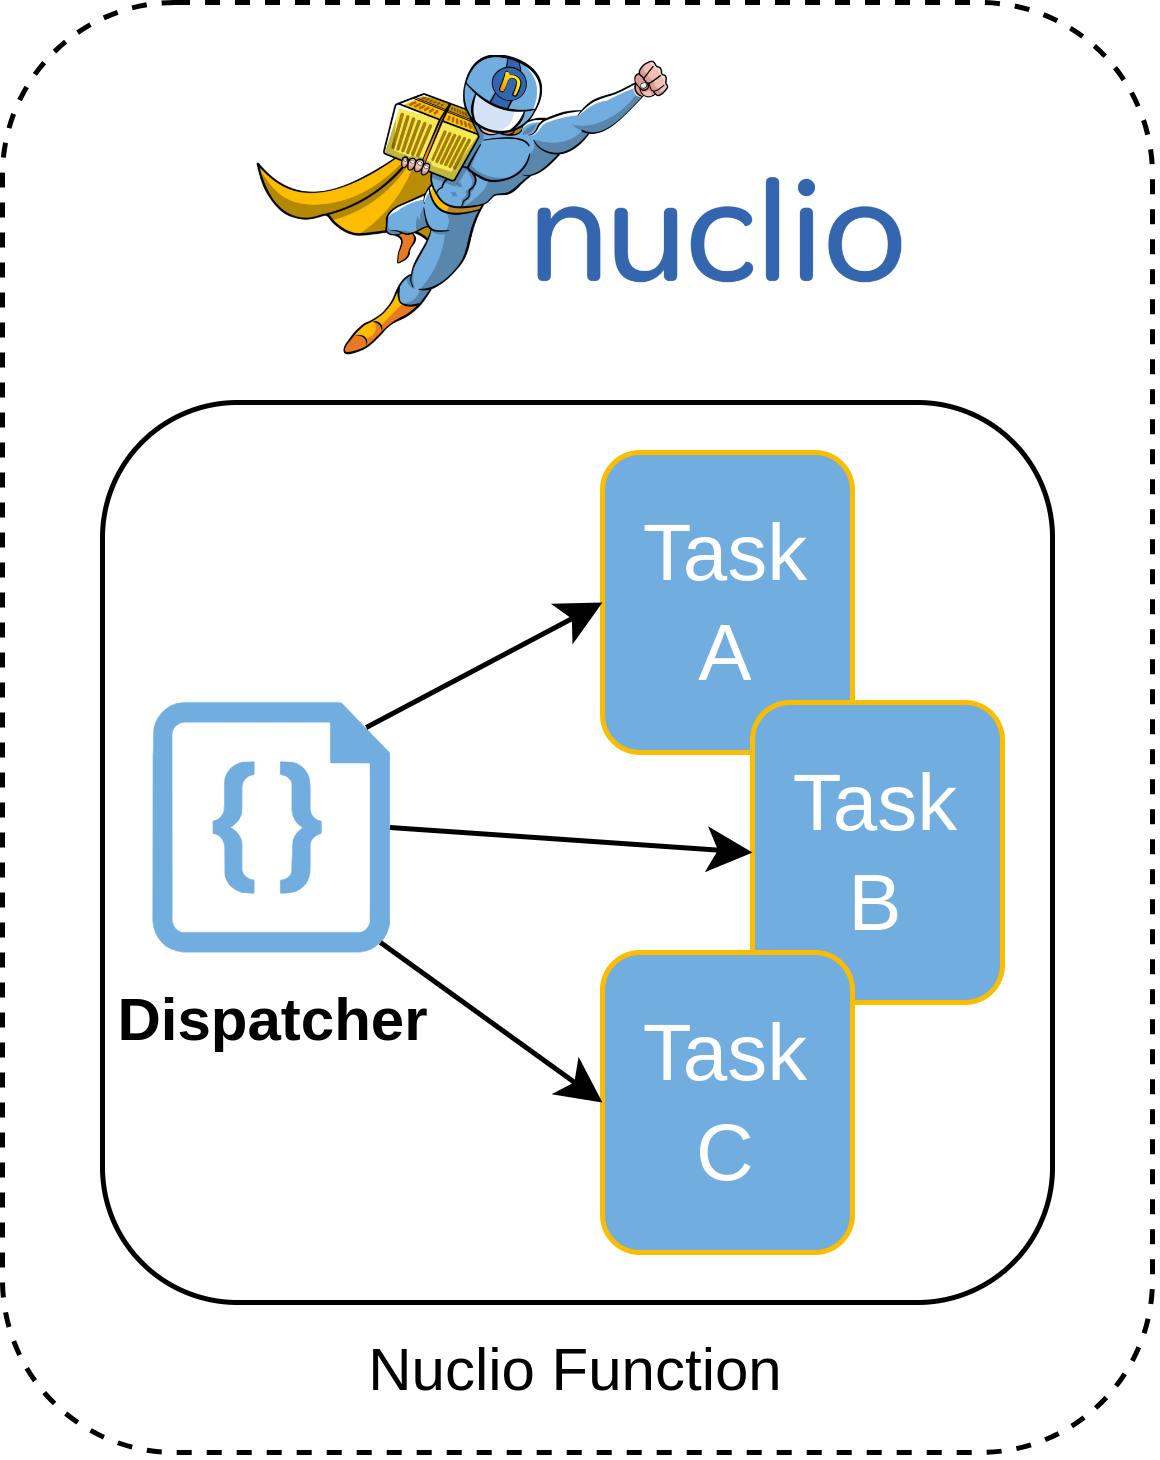
\includegraphics[width=.5\linewidth]{../figures/fusionizer_dispatcher}
    \caption{
        The Fusionizer Dispatcher routes incoming requests to the correct task
        within a Nuclio function, manages intra-group traffic, and can locally
        invoke a task if it resides within the local fusion group.
    }
    \label{fig:fusionizer_dispatcher}
\end{figure}

Figure \ref{fig:fusionizer_dispatcher} illustrates the integration of the
Fusionizer Dispatcher with a fusion group to establish a Nuclio function. The
primary role of the Dispatcher is to direct incoming requests to the appropriate
tasks. From the perspective of the exterior or from Nuclio, this appears as a
single function.

In order to pinpoint a specific task for invocation, the Fusionizer server
utilizes an HTTP header to communicate to the Dispatcher which task should
receive the request. The Dispatcher holds a secondary role of managing traffic
between tasks within the same function, or fusion group, which is crucial due to
its ability to bypass the need for routing requests across the network. This
eliminates the issues of remote call overheads and cold start cascades.

The Dispatcher achieves this through the use of a custom HTTP adapter, obtained
from the requests library. This adapter is provided to the handlers of all
tasks, which is then employed to make HTTP requests. The adapter verifies
whether the requested address is related to the Fusionizer server, and if the
target task is located within the current local fusion group. If both conditions
are met, the task request is invoked locally. Otherwise, the request proceeds as
a standard HTTP request.

\subsection{User Function Setup}

%users have to provide a handler script and a configuration YAML file
%the handler script is like previously mentioned based on Nuclio's Python
%reference. The only difference is that Fusionizer enabled Python functions need
%to have an additional parameter in their handler method called
%requests_session. This is the custom HTTP adapter as detailed in the previous
%section. When making HTTP request, users are encouraged to use this session

Users are required to supply both a handler script and a configuration YAML
file. As previously noted, the handler script should be based on Nuclio's Python
reference. However, Fusionizer-enabled Python functions need to feature an
additional parameter in their handler method named \texttt{requests\_session}.
This serves as the custom HTTP adapter that enables local task invocation
interception, as detailed in the previous section. For making HTTP requests,
users are encouraged to utilize this session. The usage of this requests session
in a handler method is outlined in Listing \ref{lst:example_handler}.

\begin{figure}
    \begin{lstlisting}[
        style=python,
        caption={
            Example handler method that showcases the usage of the custom
            requests session that is needed, when invoking other
            Fusionizer-enabled tasks.
        },
        label={lst:example_handler}
    ]
def handler(context, event, !\textbf{requests\_session}!):
    fusionizer = event.headers[
        "Fusionizer-Server-Address"
    ]
    # invoke other Task
    task = "task42"
    url = f"http://{fusionizer}:8000/{task}"
    headers = {
        "Content-Type": "application/json"
    }
    data = {"value1": 5, "value2": 3}
    # use custom requests session
    response = !\textbf{requests\_session}!.post(
        url,
        headers=headers,
        json=data
    )
    return response.text
    \end{lstlisting}
\end{figure}

%setup of the YAML configuration file stays the same. Users only need to watch
%out for compatibility across tasks since the Nuclio function they are deployed
%with only has one configuration. Tasks are therefore e.g. incompatible when:
%- they have the same dependencies with different versions
%- have different min and max replica count
%- cpu limitations
% A tasks description is also omitted in favor for its fusion group's
% description

The setup of the YAML configuration file remains consistent. Users must simply
be mindful of task compatibility due to the fact that the Nuclio function within
which they are deployed only has a single configuration. Consequently, tasks can
become incompatible under certain conditions such as sharing the same
dependencies but with varying versions, having diverse minimum and maximum
replica counts, or possessing differing CPU limitations. A task's description is
also excluded, in favor for the description of its fusion group.
